\begin{figure*}[htp]
  \centering
  \begin{subfigure}[b]{0.475\textwidth}
      \centering
      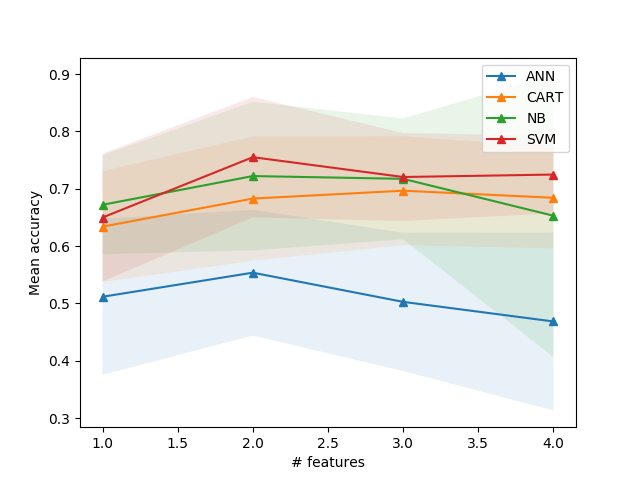
\includegraphics[width=\textwidth]{../plots_with_std_fill/Cleaned_data_sb_combined.png}
      \caption[]%
      {{\small}}
      \label{fig:EN_sbs}
  \end{subfigure}
  \hfill
  \begin{subfigure}[b]{0.475\textwidth}
      \centering
      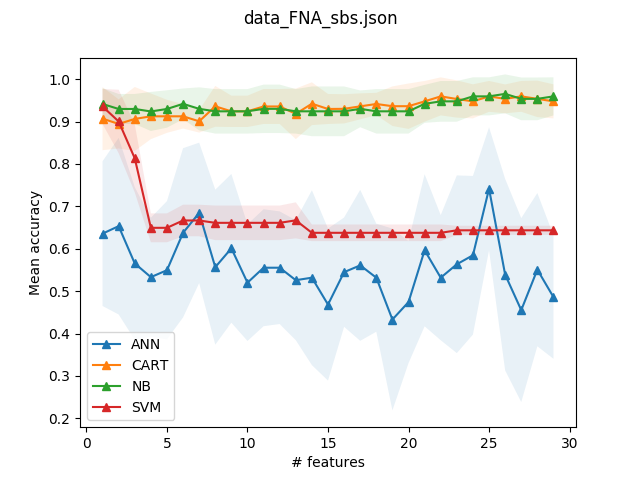
\includegraphics[width=\textwidth]{../plots_with_std_fill/data_FNA_sb_combined.png}
      \caption[]%
      {{\small}}
      \label{fig:WBCD_sbs}
  \end{subfigure}
  \vskip\baselineskip
  \begin{subfigure}[b]{0.475\textwidth}
      \centering
      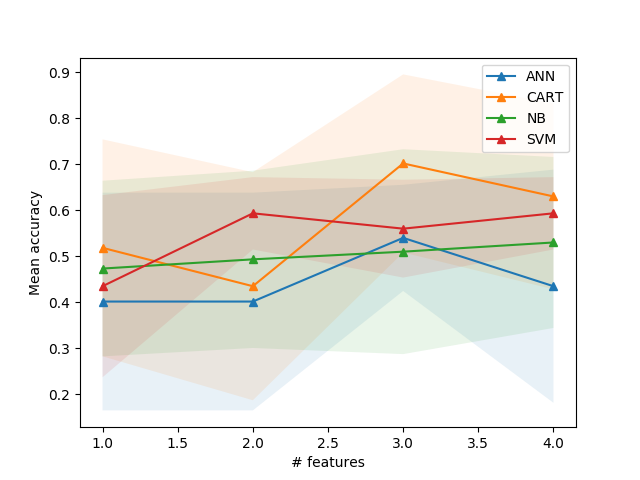
\includegraphics[width=\textwidth]{../plots_with_std_fill/Data_mias_sb_combined.png}
      \caption[]%
      {{\small}}
      \label{fig:MIAS_sbs}
  \end{subfigure}
  \quad
  \begin{subfigure}[b]{0.475\textwidth}
      \centering
      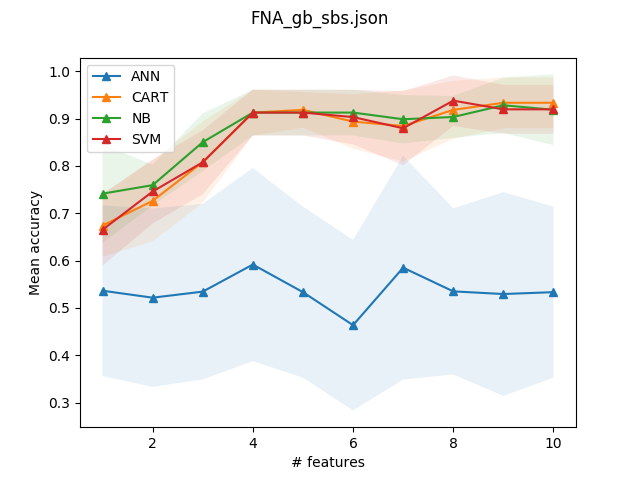
\includegraphics[width=\textwidth]{../plots_with_std_fill/FNA_gb_sb_combined.png}
      \caption[]%
      {{\small}}
      \label{fig:RHH_sbs}
  \end{subfigure}
  \caption[]
  {{\small (a) Dataset EN using SBS. (b) Dataset WBCD using SBS. (c) Dataset MIAS using SBS. (d) Dataset RHH using SBS. Combined plots of all datasets comparing each classifier when using SBS for feature selection.}}
  \label{fig:plots_sbs}
\end{figure*}
